\chapter{Постановка задачи}

    Из-за наличия разных представлений одних и тех же знаний наряду с проблемой соответствия этих представлений друг другу встает задача преобразования одних представлений в другие.
 
    В данной дипломной работе предполагается создать программное средство, которое будет автоматизировать преобразование представлений знаний систем планирования из текстового (PDDL-представления) в графическое (в виде UML-моделей).
 Получение UML-представления может быть полезно, так как:
    \begin{itemize}
        \item UML-модели более наглядны, составлять UML базы знаний могут эксперты, не знакомые с PDDL;
        \item UML-модель может быть отредактирована в UML-редакторе, и при необходимости её можно транслировать в другие языки (Java, PDDL, и~др.);
        \item существуют средства валидации и исполнения UML-моделей для проверки корректности знаний\cite{use}; 
        \item существуют средства трансформации моделей, с помощью которых можно из UML-модели предметной области получить описания задач для этой предметной области.
    \end{itemize}

   \par  Пусть $K$~--- знания системы планирования, $K = \langle D, T \rangle$, где $D$~--- знания о предметной области,
    $T = \{t_1, t_2, ...\}$~--- условия задач для данной предметной области.
 Знания о предметной области в свою очередь могут быть представлены в виде $D = \langle Types, Relations, Actions \rangle$, где $Types$~--- знания о типах объектов предметной области, $Relations$~--- знания о типах отношений между объектами, $Actions = {a_1, a_2, ...}$~--- знания о действиях $a_i$.
 Действие представляется в виде $a_i = \langle partypes, precond, effect \rangle$ и состоит из знаний о типах параметров, знаний о предусловии действия и эффекте от его применения.
 Типы параметров~--- упорядоченная последовательность типов $ partypes = \langle c_1, c_2, ..., c_n \rangle, c_i \in Types$.
 Действие $a$ применимо в том и только том состоянии $s$ для которого $precond_a(s,p) = True, s \in S, p \subset s$, где $S$~--- пространство всех состояний, $p = \langle o_1, o_2, ..., o_n \rangle$~--- фактические параметры действия с соответствующими типами.
 Эффект действия фактически задает новое состояние: $effect_a(s, p) = s' \in S$.
 Задачи представляются в виде $t_i = \langle Init, Goal \rangle$, где $Init \in S$~--- начальное состояние, $Goal: S \rightarrow \mathbb{B}$~--- ограничения на целевое состояние, отображение состояний в булево множество $\mathbb{B} = \{ True, False\}$.
 Любое состояние $s \in S$ представляется знаниями об объектах (экземплярах типа) и об отношениях между ними (экземпляры отношений), что иначе называется конфигурацией объектов и отношений, т.е.
 $s = \{o_1, o_2, ..., o_n, rel_1, rel_2, ..., rel_m\}$, $o_i$~--- экземпляр типа из $Types$, $rel_j$~--- экземпляр отношения из $Relations$.
    
    Знания в PDDL-представлении задаются следующим образом.
 $D_{PDDL} = \langle Types_{PDDL}, Relations_{PDDL}, Actions_{PDDL} \rangle$, где $Types_{PDDL}$~--- описания типов, $Relations_{PDDL}$~--- описания отношений в виде предикатов, $Actions_{PDDL}$~--- описания параметров действий, их предусловий и эффектов.
 Задачи  $t_{i, PDDL} = \langle Init_{PDDL}, Goal_{PDDL} \rangle$ описываются перечислением объектов с их типами, уточнением отношений между объектами.
   Все это можно увидеть на примере, приведенном раннее.
    
    Знания в UML-представлении можно задать следующим образом в виде модели UML.
  $D_{UML} = \langle Types_{UML}, Relations_{UML}, Attributes_{UML}, Actions_{UML} \rangle$, где $Types_{UML}$~--- UML-классы, соответствующие PDDL-типам, $Relations_{UML}$~--- UML-ассоциации между классами, соответствующие \textit{n-арным} ($n > 1$) между типами в PDDL, $Attributes_{UML}$~--- атрибуты классов, соответствующие \textit{унарным} предикатам PDDL, $Actions_{UML}$~--- описания параметров действий, их предусловий и эффектов.
 $Types_{UML}$ и $Relations_{UML}$ могут быть промоделированы с использованием диаграмм классов.
 $Actions_{UML}$ могут быть заданы, например, при помощи OCL.
 Задачи  $t_{i, UML} = \langle Init_{UML}, Goal_{PDDL} \rangle$ описываются с помощью объектов с указанием их типов, значений атрибутов и экземпляров ассоциаций.
 Задачи могут быть промоделированы с использованием диаграмм объектов.
 Состояние в UML может быть представлено как $ s \in S_{UML}, s = \{o_1, o_2, ..., o_n, rel_1, rel_2, ..., rel_m, atr_1, atr_2, ..., atr_l\}$, где $atr_i$~--- экземпляры атрибутов.
    
    В ходе работы создаваемого средства к представлению будет применяться ряд преобразований.
  За основу этих преобразований предполагается взять предложенное в работе \cite{mal-manz} преобразование UML-моделей в PDDL.
 Семантика знаний при преобразовании представлений должна сохраняться.
     
    Вышесказанное можно формализовать следующим образом.
 Пусть $F$~--- описываемое преобразование, $F: K_{PDDL} \to K_{UML}$, $K_{PDDL}$~--- знания в исходном (текстовом PDDL-представлении), $K_{UML}$~--- база знаний в целевом представлении (в виде UML-модели).
 Преобразование $F$ можно представить в виде композиции преобразований $F = \langle F_T, F_R, F_A, F_C \rangle$, где $F_T: Types_{PDDL} \rightarrow Types_{UML}$~--- преобразование типов, $F_R: Relations_{PDDL} \rightarrow Relations_{UML} \cup Attributes_{UML}$~--- преобразование отношений, $F_A: Actions_{PDDL} \rightarrow Actions_{PDDL}$~--- преобразование действий, $F_C: t_{i, PDDL} \rightarrow t_{i, UML}$~--- преобразование задач.
 Преобразования должны обладать следующими свойствами:
    
    \begin{enumerate}
        \item В отображении типов (Рис.
~\ref{img:property-types}) $F_T$ любому PDDL-типу должен соответствовать UML-класс, причем, разным типам должны соответствовать разные классы.
 Если типы связаны отношением тип-подтип, то в UML между ними должна быть связь обобщения:
    
        \begin{center}
            $\forall c \in Types_{PDDL} \Rightarrow F_T(c) \in Types_{UML}$; \\
            $\forall c_1, c_2 \in Types_{PDDL}, c_1 \neq c_2 \Rightarrow F(c_1) \neq F(c_2)$;
        \end{center}
                 
        
\begin{figure}[!h]
    \hfill
    \begin{minipage}[h]{0.40\linewidth}
        {\raggedright
        \begin{verbatim}
    (:types
        thing - object
        stone - thing
    )
        \end{verbatim} 
        }
    \end{minipage}
    \hfill
    $\rightarrow$
    \hfill
    \begin{minipage}[h]{0.45\linewidth}
        \center{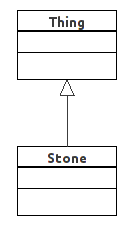
\includegraphics[width=0.5\linewidth]{property-types}}
    \end{minipage}
    \caption{Пример преобразования типов}
    \label{img:property-types}
\end{figure}
   

        \item В отображении отношений (Рис.~\ref{img:property-relations}) $F_R$ любому PDDL-предикату соответствует ассоциация UML либо атрибут UML-класса.
 Причем, если предикат \textit{унарный}, то он отображается в атрибут, иначе в ассоциацию; также разным предикатам соответствуют разные ассоциации/атрибуты:
    
        \begin{center}
        $\forall rel \in Relations_{PDDL} \Rightarrow F_R(rel) \in Relations_{UML} \cup Attributes_{UML}$;\\
        $\forall rel_1, rel_2 \in Relations_{PDDL}, rel_1 \neq rel_2 \Rightarrow F_R(rel_1) \neq F_R(rel_2)$; \\
        \end{center}

    
\begin{figure}[h]
    \hfill
    \begin{minipage}[h]{0.50\linewidth}
        {\raggedright
        \begin{verbatim}
    (:predicates
      (right ?phi - Philosopher 
          ?for - Fork)
      (hungry ?phi - Philosopher)
    )
        \end{verbatim} 
        }
    \end{minipage}
    \hfill
    $\rightarrow$
    \hfill
    \begin{minipage}[h]{0.45\linewidth}
        \center{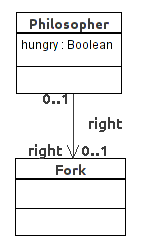
\includegraphics[width=0.5\linewidth]{property-relations}}
    \end{minipage}
    \caption{Пример преобразования отношений}
    \label{img:property-relations}
\end{figure}       


        \item 
        Введем вспомогательное отображение объектов в соответствующие типы $Type: o \in S \rightarrow Types$, отображение экземпляров отношений в соответствующие типы отношений $Relation: rel \in S \rightarrow Relations$, отображение экземпляров атрибутов в соответствующие атрибуты $Attribute_{UML}: atr \in S_{UML} \rightarrow Attributes_{UML}$, и отображение состояний $F_S: S_{PDDL} \rightarrow S_{UML}$,  для корректного определения которого потребуем выполнения следующих свойств:
       \begin{center}
        $\forall s = \{ o_1, ..., o_n, rel_1, ..., rel_m \} \in S_{PDDL} \Rightarrow$ \\ 
        $\Rightarrow F_S(s) = \{ o_1', ..., o_n', rel_1', ..., rel_k', atr_1, ..., atr_k \} \in S_{UML}$;  \\
                
        $\forall o_i \in s \Rightarrow F_T(Type_{PDDL}(o_i)) = Type_{UML}(o_i') $; \\  
        $\forall rel_i \in s \Rightarrow F_R(Relation_{PDDL}(rel_i)) = $
\[ = \left\{ 
    \begin{array}{l l}
        Attribute_{UML}(rel_k') & \quad \text{, $Relation_{PDDL}(rel_i)$~--- унарный предикат;} \\
        Relation_{UML}(atr_l) & \quad \text{, иначе;}
    \end{array}     
\right.\]
        \end{center}
        
        Тогда отображение задач (Рис.~\ref{img:property-tasks}) $F_C$ должно обладать следующим свойством корректности относительно отображения $F_S$ :
        
        \begin{center}
            $\forall t = \langle I, G \rangle \in T_{PDDL} \Rightarrow F_C(t) = \langle F_S(I), G' \rangle$; \\
            $\forall s \in S_{PDDL} \Rightarrow G(s) = True \Leftrightarrow G'(F_S(s)) = True $
        \end{center}
   
\begin{figure}[h]
    \center{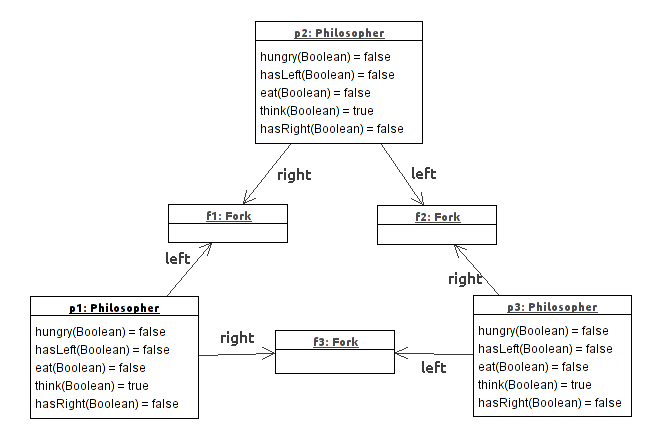
\includegraphics[width=1\linewidth]{property-tasks}}
    \caption{Пример преобразования состояний}
    \label{img:property-tasks}
\end{figure}   
           
        \item
    Отображение действий (Рис.
~\ref{img:property-actions}) $F_A$ должно удовлетворять следующим требованиям:
    \begin{center}
        $\forall a \in Actions_{PDDL} \Rightarrow F_A(a) \in Actions_{UML}$; \\    
    
        $\forall a_1, a_2 \in Actions_{PDDL}, a_1 \neq a_2 \Rightarrow F_A(a_1) \neq F_A(a_2)$; \\        
 
        $\forall a \in Actions_{PDDL}, partypes_a = \langle c_1, c_2, ..., c_n \rangle \Rightarrow F_A(a) = a', partypes_{a'} = \langle F_T(c_1), F_T(c_2), ..., F_T(c_n)\rangle$; \\
 
        $\forall a \in Actions_{PDDL}, \forall s \in S_{PDDL}, a' = F_A(a) \Rightarrow precond_a(s, p) = True, p \subset s \Leftrightarrow precond_{a'}(F_S(s), p') = True, p' = F_S(p)$, и \\
        
        $effect_{a'}(F_S(s), p') = F_S(effect_a(s, p)), p \subset s, p' = F_S(p) $;
    \end{center}            
       
\begin{figure}[h]
    \begin{minipage}[h]{1\linewidth}
        \center{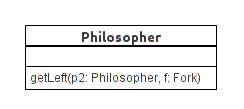
\includegraphics[width=0.5\linewidth]{property-actions}}    
    \end{minipage} \\
    \vfill
    {\centering $+$ \\ \medskip } 
        \begin{minipage}[h]{0.43\linewidth}
        
           \begin{verbatim}
    context Philosopher::getLeft(p2: Philosopher, f: Fork)
        pre 
            self.left = f 
            and p2.right = f 
            and self.hungry 
            and not p2.hold->includes(f)
        post
            self.hasLeft
            and self.hold = self.hold@pre->including(f)
            and not self.hungry
           \end{verbatim}
        \end{minipage}

    \begin{center}
        \begin{minipage}{0.8\linewidth}
            \caption{Один из вариантов преобразования действий с ограничениями на OCL на примере $getLeft$ }
        \end{minipage}    
    \end{center}

    \label{img:property-actions}
\end{figure}      

    \item
        Планом, решающим задачу $t = \langle I, G \rangle$ называется последовательность 
        \begin{center}
            $\langle s_1, a_1, p_1  \rangle, \langle s_2, a_2, p_2  \rangle, ..., \langle s_N, \emptyset, \emptyset \rangle \in Plans(t)$, \\ $s_i \in S, a_i \in Actions, p_i \subset s_i$
        \end{center}
        такая, что $s_1 = I, s_i = effect_{a_{i-1}}(s_{i-1}, p_{i-1}), i > 1$ и $G(s_N) = True$ где $Plans(t)$~--- множество планов, решающих задачу $t$.
            
        Введем вспомогательное отображение планов $F_P: Plans_{PDDL}(t) \rightarrow Plans_{UML}(t)$:
            \begin{center}
                $\forall p = \langle s_1, a_1, p_1  \rangle, \langle s_2, a_2, p_2  \rangle, ..., \langle s_N, \emptyset, \emptyset  \rangle \in Plans_{PDDL}(t) \Rightarrow $\\
            $F_P(p) = \langle F_S(s_1), F_A(a_1), F_S(p_1)  \rangle, \langle F_S(s_2), F_A(a_2), F_S(p_2)  \rangle, ..., \langle F_S(s_N), \emptyset, \emptyset  \rangle \in Plans_{UML}(t) $  
            \end{center}
            
        Преобразование $F$ должно обладать свойством сохранения планов:
        
        \begin{center}
            $\forall t = \langle I, G\rangle \in T_{PDDL}, p \in Plans_{PDDL}(t) 
            \Leftrightarrow F_P(p) \in Plans_{UML}(t) $

        \end{center}
    \end{enumerate}
    

    Данное преобразование довольно легко формализовать и реализовать для PDDL-описаний, использующих только подмножество STRIPS.
 Какие возможности PDDL за пределами STRIPS может поддержать разрабатываемое средство, каким образом их представлять в UML-моделях ~--- это все еще является открытым вопросом и темой для исследований.
 Сложности могут возникнуть, например, в необходимости задания ограничений на целевое состояние с использованием кванторов, что невозможно сделать только лишь с помощью диаграмм объектов.
 Другой сложностью может быть трансляция длительных действий PDDL, например, во временные диаграммы UML.
 Существенной подзадачей является также преобразование предусловий и эффектов операций из PDDL в OCL.
 
\newpage